\item La clienta \textbf{Lena Cacioppo} compró un producto de cada subcategoría de \textbf{Furniture}. Deberás elegir los productos que desees e indicar como parte de esta consulta, la información que se agregará en cada caso.

\begin{lstlisting}
lena_customerid = π customerid (σ customername = 'Lena Cacioppo' (customer))
furniture_types = π subcategory (σ category = 'Furniture' (products))
lena_orders = {
  orderid:string, orderdate:date, shipdate:date, shipmode:string, customerid:string, productid:string, quantity:number
  'US-2026-342349', 2026-10-26, 2026-10-30, 'Same Day', 'LC-16870', 'FUR-BO-10001798', 1
	'US-2026-342349', 2026-10-26, 2026-10-30, 'Same Day', 'LC-16870', 'FUR-CH-10000454', 1
	'US-2026-342349', 2026-10-26, 2026-10-30, 'Same Day', 'LC-16870', 'FUR-TA-10000577', 1
	'US-2026-342349', 2026-10-26, 2026-10-30, 'Same Day', 'LC-16870', 'FUR-FU-10001487', 1
}

orders U lena_orders
\end{lstlisting}

\begin{center}
  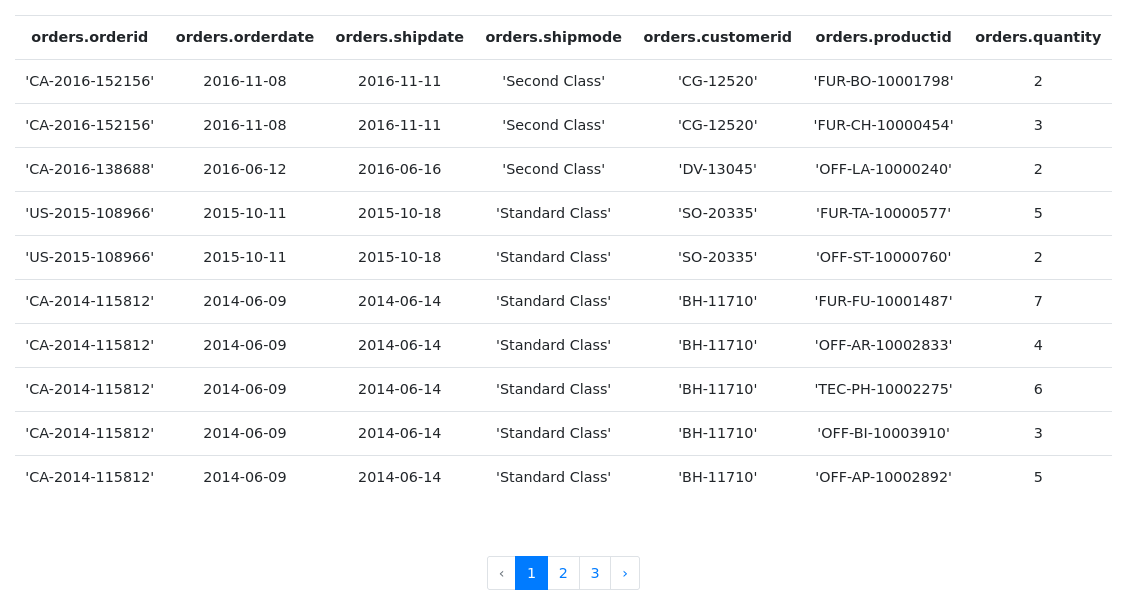
\includegraphics[width=0.7\textwidth]{figuras/3c_1.png}
\end{center}

\begin{center}
  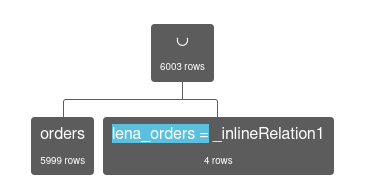
\includegraphics[width=0.7\textwidth]{figuras/3c_2.png}
\end{center}
